\chapter{Аналитическая часть}

\section{Сущности предметной области}

Основными сущностями предметной области являются:
\begin{itemize}
	\item игра --- программа для которой создаются модификации;
	\item категория --- категория, к которой может относиться модификация;
	\item модификация --- набор различных версий модификаций;
	\item версия модификации --- определенная версия некоторой модификации;
	\item файл модификации --- определенный файл некоторой версии модификации;
	\item пользователь --- человек, использующий платформу;
	\item комментарий --- текст, который пользователь оставляет к модификации;
	\item подборка --- множество сгруппированных пользователем модификаций.
\end{itemize}

\section{Сравнение аналогичных решений}

Критерии сравнения:
\begin{itemize}
	\item К1 --- возможность скачивать модификации без регистрации;
	\item К2 --- возможность создания пользовательских наборов модификаций;
	\item К3 --- наличие обратной связи у создателей модификаций (комментарии).
\end{itemize}

Сравнение было приведено в таблице~\ref{tab:comp}.
\begin{table}[H]
	\centering
	\caption{Таблица сравнения аналогичных сервисов}
	\label{tab:comp}
	\begin{tabularx}{\textwidth}{|X|X|X|X|}
		\hline
		\textbf{Сервис} & \textbf{К1} & \textbf{К2} & \textbf{К3} \\
		\hline
		Nexus Mods & $-$ & $+$ & $+$ \\
		\hline
		CurseForge & $+$ & $-$ & $+$ \\
		\hline
		Modrinth & $+$ & $+$ & $-$ \\
		\hline
	\end{tabularx}
\end{table}

При сравнении аналогичных решений было выявлено, что ни один из рассмотренных сервисов не обладает всеми выбранными функциональными возможностями одновременно, поэтому разрабатываемая система должна объединять их в рамках единой платформы.

\section{Требования, предъявляемые к разрабатываемому сервису}

\subsection*{Акторы}

\begin{itemize}
	\item гость --- неавторизованный пользователь, который может просматривать и скачивать модификации других пользователей;
	\item авторизованный пользователь --- аналогично гостю, но может выкладывать свои модификации и оставлять отзывы на модификации других пользователей.
	\item администратор --- занимается модерацией выложенных пользователями модификаций, изменение справочной информации.
\end{itemize}

\subsection*{Функциональные требования}

Необходимо предоставить возможность:
\begin{itemize}
	\item пользователям выкладывать собственные модификации и оставлять комментарии на чужих модификациях;
	\item скачивать модификации, в том числе неавторизованным пользователям;
	\item пользователям составлять собственные подборки модификаций;
	\item администрации проводить модерацию выложенных модификаций;
	\item производить поиск модификаций с помощью различных фильтров.
	
\end{itemize}

\subsection*{Ограничения}

\begin{itemize}
	\item максимальный размер одного файла --- 100 МБ;
	\item максимальное количество файлов для одной версии модификации --- 5;
	\item максимальный размер изображения модификации --- 3 МБ;
	\item допустимые форматы для изображений --- png, svg, jpg, jpeg;
	\item модификация обязательно должна относиться к какой-либо игре;
	\item у модификации обязательно должна быть хотя бы одна версия.
\end{itemize}

\section{Диаграмма прецедентов}

В соответствии с выделенными акторами и предъявленными требованиями была составлена диаграмма прецедентов платформы. Диаграмма представлена на рисунке~\ref{diag:use-case}. Она отражает основные сценарии взаимодействия пользователей с системой и демонстрирует ключевые функциональные возможности платформы. На основе данной диаграммы были определены основные требования к реализации пользовательского и административного функционала.

\begin{figure}[H]
	\centering
	
\includegraphics[width=0.7\textwidth]{use-case}
	\caption{Диаграмма прецедентов}
	\label{diag:use-case}
\end{figure}

\section{Диаграмма <<сущность--связь>>}

Диаграмма <<сущность--связь>> в нотации Чена необходима для концептуального моделирования предметной области до перехода к конкретной базе данных~\cite{chen}. Сделанная на основе анализа предметной области диаграмма представлена на рисунке~\ref{diag:er}. Она отражает основные сущности системы, их атрибуты и взаимосвязи между ними. Полученная модель служит основой для дальнейшего проектирования структуры базы данных и её логической схемы.

\begin{figure}[H]
	\centering
	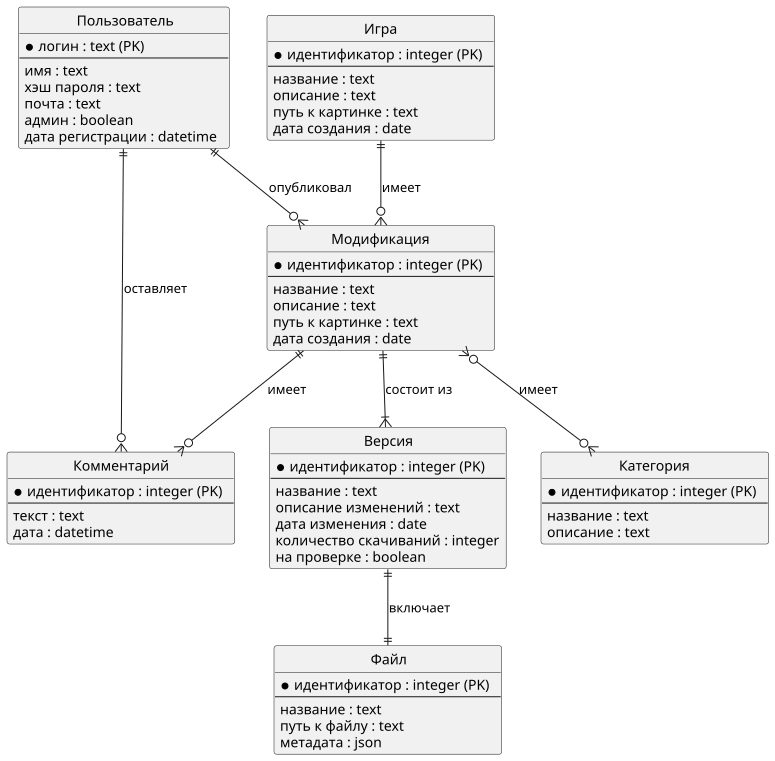
\includegraphics[width=\textwidth]{er}
	\caption{Модель <<сущность--связь>>}
	\label{diag:er}
\end{figure}

\section{Анализ моделей хранения данных}

Модель данных представляет собой логическую структуру, определяющую правила организации, хранения и манипулирования данными в информационной системе~\cite{avrunev}. 

\subsection{Дореляционные модели данных}

К дореляционным моделям относятся иерархическая и сетевая модели. Характерной чертой данных моделей является навигационный принцип доступа к данным, при котором логика перемещения по записям реализуется на уровне прикладного программного обеспечения~\cite{avrunev}.

\subsubsection{Иерархическая модель}
Иерархическая модель строится по принципу древовидного графа. Объекты связаны отношениями типа <<один ко многим>> ($1:N$), где каждый <<потомок>> может иметь только одного <<предка>>.
\begin{itemize}
	\item к преимуществам модели относится высокая скорость доступа к данным при поиске по вертикальным связям за счет использования физических указателей;
	\item к недостаткам следует отнести избыточность данных при попытке реализации связей типа <<многие ко многим>> ($M:N$), а также жесткую зависимость данных: удаление родительского объекта влечет за собой автоматическое удаление всех подчиненных записей~\cite{avrunev}.
\end{itemize}

\subsubsection{Сетевая модель}
Сетевая модель является расширением иерархической и допускает наличие у одного объекта нескольких <<предков>>, что позволяет напрямую описывать отношения типа $M:N$.
\begin{itemize}
	\item преимуществом модели является отсутствие дублирования данных, характерного для иерархического подхода;
	\item основной недостаток заключается в высокой сложности схемы и трудоемкости разработки, обусловленной необходимостью явного описания путей навигации по связям-указателям между записями~\cite{avrunev}.
\end{itemize}

\subsection{Реляционная модель данных}

Реляционная модель, предложенная Э. Коддом, базируется на математической теории множеств и логике предикатов. Данные представляются в виде совокупности нормализованных отношений (таблиц)~\cite{avrunev}.

В отличие от навигационных моделей, реляционный подход использует декларативный язык запросов SQL. К ключевым характеристикам модели, согласно правилам Кодда, относятся:
\begin{itemize}
	\item целостность сущностей и ссылочная целостность, реализуемые через механизмы первичных и внешних ключей;
	\item логическая и физическая независимость данных: возможность изменения структуры хранения или описания данных без переработки прикладного ПО;
	\item минимизация избыточности: за счет приведения таблиц к нормальным формам реляционная модель исключает аномалии вставки, обновления и удаления данных~\cite{codd, avrunev, kuznetsov}. 
\end{itemize}

\subsection{Постреляционные модели хранения данных}

Парадигма NoSQL ориентирована на решение задач горизонтального масштабирования и обработки неструктурированных данных. В отличии от реляционной модели в постреляционных моделях используется денормализация для повышения скорости доступа к данным~\cite{avrunev}.

\subsubsection{Модель <<ключ-значение>>}
Данная модель представляет собой ассоциативное хранилище, где доступ к данным осуществляется по уникальному идентификатору (ключу).
\begin{itemize}
	\item основным достоинством является минимальное время отклика, не зависящее от объема хранимой информации;
	\item ограничением модели является отсутствие механизмов контроля связей и невозможность выполнения выборок по содержимому хранимых значений~\cite{avrunev, komarov}.
\end{itemize}

\subsubsection{Документная модель}
Модель <<ключ-значение>>, где значением является документ.
В рамках данной модели данные хранятся в виде структурированных документов (например, в формате JSON, CSV и т.д.), обладающих собственной внутренней иерархией.
\begin{itemize}
	\item преимуществом модели является гибкость схемы данных и возможность хранения связанных объектов внутри одного документа;
	\item к недостаткам относится низкая скорость выполнения операций объединения (JOIN) между различными коллекциями, что требует реализации логики связывания на уровне приложения~\cite{avrunev, komarov}.
\end{itemize}

\subsection{Сравнительный анализ моделей данных}

Для объективного выбора архитектуры хранения данных необходимо провести сравнение рассмотренных моделей по ключевым техническим критериям (К1--К5):
\begin{itemize}
	\item К1 --- обеспечение строгой ссылочной целостности на уровне СУБД;
	\item К2 --- наличие декларативного языка запросов (SQL и аналоги);
	\item К3 --- поддержка связей типа <<многие ко многим>> ($M:N$) без дублирования данных;
	\item К4 --- отсутствие аномалий вставки, обновления и удаления за счет механизмов нормализации;
	\item К5 --- возможность горизонтального масштабирования системы.
\end{itemize}

Результаты сравнительного анализа представлены в таблице~\ref{tab:models_comp}.

\begin{table}[H]
	\centering
	\caption{Сравнительная характеристика моделей хранения данных}
	\label{tab:models_comp}
	\begin{tabularx}{\textwidth}{|l|X|X|X|X|X|}
		\hline
		\textbf{Модель данных} & \textbf{К1} & \textbf{К2} & \textbf{К3} & \textbf{К4} & \textbf{К5} \\
		\hline
		Иерархическая & $-$ & $-$ & $-$ & $-$ & $-$ \\
		\hline
		Сетевая & $-$ & $-$ & $+$ & $-$ & $-$ \\
		\hline
		\textbf{Реляционная} & $+$ & $+$ & $+$ & $+$ & $+/-$ \\
		\hline
		Ключ-значение & $-$ & $-$ & $-$ & $-$ & $+$ \\
		\hline
		Документная & $+/-$ & $+/-$ & $-$ & $-$ & $+$ \\
		\hline
	\end{tabularx}
\end{table}

\subsection{Обоснование выбора модели}

Проведенный анализ предметной области выявил наличие множества взаимосвязанных сущностей (пользователи, модификации, файлы) с преобладанием связей типа $M:N$. Применение дореляционных моделей нецелесообразно ввиду высокой сложности поддержки навигационных путей доступа. Использование документных NoSQL-моделей приведет к нарушению целостности данных из-за отсутствия механизмов связывания объектов.

На основании изложенного, для реализации основного хранилища системы была выбрана реляционная модель данных, поскольку она обеспечивает требуемый уровень ссылочной целостности.

Для оптимизации производительности при обработке часто запрашиваемых данных (кэширование сессий, самых частых запросов) необходимо использовать вспомогательное хранилище типа <<ключ--значение>>. Данный комбинированный подход позволяет сочетать транзакционную надежность реляционной СУБД с высокой скоростью доступа NoSQL-решения.

\section{Вывод}

В аналитической части проанализированы различные модели хранения данных, а также построена диаграмма <<сущность--связь>> предметной области в нотации Чена. В результате анализа было принято решение использовать реляционную модель для основного хранения данных платформы модификаций, так как она удобно описывает связи между играми, модификациями, версиями, файлами и пользователями, а также обеспечивает поддержку сложных запросов и ссылочной целостности.  

Дополнительно к реляционной модели планируется использовать хранилище типа <<ключ--значение>> для кэширования часто запрашиваемых данных. Это позволит снизить нагрузку на основную базу и ускорить отклик сервиса.

\clearpage
